\documentclass[../../Cours_M1.tex]{subfiles}
\newcommand{\nomTD}{TP4 : Asservissement par retour d'état}
\renewcommand{\nomentete}{UE421-\nomTD}
\renewcommand{\auteur}{Aymeric Arnould, Tom Colinot}
\newcommand{\z}{z^{-1}}

\title{TP4 : Asservissement de position d'un moteur à courant continu par retour d'état}
\author{\auteur}

\begin{document}
\maketitle

\section*{I/ Introduction}
Nous allons dans ce TP mener une première étude pour identifier le moteur considéré. Ensuite, nous mettrons en place une correction proportionnelle, afin de voir dans quelle mesure la correction par retour d'état permet un meilleur réglage des paramètres du système bouclé.


\section*{II/ Présentation du moteur}

\subsection*{Préparation 1}
\begin{itemize}\setlength{\itemsep}{10mm}
\item Le frottement sec est assimilable à une perturbation en couple constant. Ainsi, pour réduire son importance dans la modélisation, il faut essayer d'augmenter l'amplitude de la tension d'entrée, et donc du couple créé, pour que celui-ci soit prépondérant devant le frottement sec. Il faut toutefois conserver une tension d'entrée entre $\pm$ 10 V pour ne pas avoir de saturation.

\item \textbf{Détermination de $K_2$}

En boucle ouverte, la fonction de transfert relative à la tension image de la position est : 
\[\frac{V_{\theta}(p)}{U(p)} = \frac{K_2}{p(1+\tau p)} = \frac{K_2}{p}-\frac{K_2\tau}{1+\tau p}\]
On en déduit la réponse indicielle :
\[v_{\theta}(t) = K_2(t -  \tau(1-e^{t/\tau})), \forall t>0\]
\begin{figure}[h!]
\centering
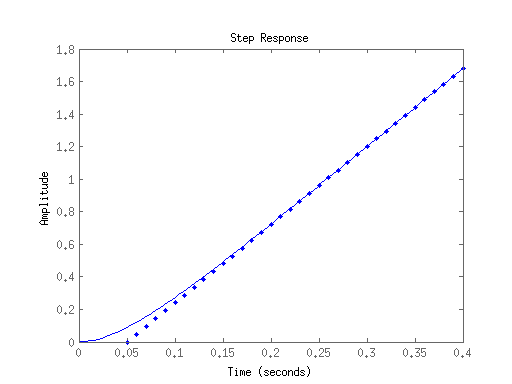
\includegraphics[scale=0.5]{indBO.png}
\caption{Allure de la réponse indicielle en boucle ouverte}
\end{figure}

Dans la réponse indicielle, $K_2$ et $\tau$ correspondent à la pente et au pied de l'asymptote.

\item \textbf{Détermination de} $K_1=KK_{\Omega}$ et $\tau$

En boucle ouverte, la fonction de transfert relative à la tension image de la vitesse est : 
\[\frac{V_{\Omega}(p)}{U(p)} = \frac{K_1}{1+\tau p} \]
On en déduit la réponse indicielle :
\[v_{\Omega}(t) = K_1(1-e^{t/\tau}), \forall t>0\]

$K_1$ est alors la valeur finale de $v_{\Omega}(t)$ et  $\tau$ est le temps de montée à $63\%$.
\end{itemize}


\subsection*{Manipulation 1}
\begin{itemize}\setlength{\itemsep}{10mm}
\item \textbf{Détermination de $K_2$} avec $v_{\theta}(t)$

On génère un créneau en entrée de la boucle ouverte. La réponse de $V_{\theta}$ donnée en \emph{Annexe 1} est une rampe. Sa pente est de 18,9 V/rad pour un échelon d'amplitude 4V. Ainsi, on a \[\boxed{K_2 = KK_{\theta} = 4,725 V/rad} \].

Déterminer $\tau$ avec cet essai ne serait pas très précis, on utilise donc le second.

\item \textbf{Détermination de} $K_1=KK_{\Omega}$ et $\tau$ avec $v_{\Omega}(t)$

On prend le même créneau mais on observe la réponse de $v_{\Omega}(t)$ donnée en \emph{Annexe 2}. On obtient un premier ordre si on prend une amplitude suffisamment grande et que l'on ajoute un offset pour que le sens de rotation ne s'inverse pas à chaque créneau.

Pour un échelon de 3V, la valeur finale est de 4V, donc \[\boxed{K_1 = KK_{\Omega} = 1,3}\]

Le temps de montée à $63\%$ est \[\boxed{\tau = 56ms}\]

\item \textbf{Essai harmonique}

On génère une tension d'entrée sinusoïdale. En observant 
\[V_{\Omega}(p) = \frac{K_1}{1+\tau p} U(p)\]
on peut déterminer $\tau$ en observant le déphasage entre $v_{\Omega}(t)$ et $u(t)$ (\emph{Annexe 3}). En effet, lorsque la pulsation vaut $\frac{1}{\tau}$, le déphasage entre les deux signaux sera de $45^o$.

On a un déphasage de $45^o$ pour une pulsation de 2,84 Hz, soit $\tau = 56ms$.

\item \textbf{Détermination de $K_{\theta}$}

Pour obtenir la valeur de $K_{\theta}$, on choisit de faire tourner le moteur d'un angle de $2\pi$ (repéré entre deux remises à zéro du capteur). Pour cela, on injecte une consigne continue (échelon de fréquence très faible). Pour $\theta$ allant de 0 à $2\pi$, la tension varie proportionnellement de $0$ à $25V$. 
On a donc
\[K_{\theta} = \frac{25}{2\pi} = 3.98 V/rad\]

On en déduit donc :
\begin{itemize}
\item $K_{\theta} = 3.98 V/rad$
\item $K = 1,18 V^{-1}.rad.s^{-1}$
\item $K_{\Omega} = 1,1V.rad^{-1}.s$
\end{itemize} 


\end{itemize}


\section*{III/ Asservissement de position par un correcteur proportionnel}

\subsection*{Préparation 2}
\begin{figure}[h!]
\centering
\begin{tikzpicture}
\sbEntree{E}
\sbComp{comp}{E}                
\sbRelier[$E(p)$]{E}{comp}

\sbBloc[3]{CP}{$C$}{comp}
\sbRelier[$U(p$)]{comp}{CP}

\sbBloc[3]{mot}{$\frac{K}{1+\tau p}$}{CP}  
\sbRelier{CP}{mot}

\sbBloc[3]{int}{$\frac{1}{p}$}{mot}      
\sbRelier[$\Omega(p)$]{mot}{int}

\sbBloc[3]{sys}{$K_{\theta}$}{int}
\sbRelier[$\theta(p)$]{int}{sys}

\sbSortie[3]{S}{sys}                
\sbRelier[$V_{\theta}(p)$]{sys}{S}

\sbRenvoi{sys-S}{comp}{}
\end{tikzpicture}
\caption{Asservissement considéré}
\end{figure}

\begin{itemize}\setlength{\itemsep}{10mm}
\item La fonction de transfert en boucle fermée est :
\[\frac{V_{\theta}(p)}{E(p)} = \frac{1}{p(1+\tau p) + K_2C} = \frac{1}{\frac{\tau}{K_2C}p^2 + \frac{1}{K_2C}p+1}\]

On en déduit donc
\begin{align*}
\omega_{0BF} & = \sqrt{\frac{K_2C}{\tau}} \\
m_{BF} & = \frac{1}{2\sqrt{\tau K_2C}} \\
C & = \frac{1}{4m_{BF}^2K_2\tau}
\end{align*}

\item On veut régler le coefficient d'amortissement $m_{BF}=0,8$. On a donc :
\[ \boxed{ C_0 = 1,63 \quad \et \quad \omega_{0BF} = 12,5 rad/s} \]

\item Les pôles de la fonction de transfert en boucle fermée $\frac{V_{\theta}(p)}{E(p)}$ sont :

\begin{multicols}{2}
Pour $m<1$
\[p_{1,2} = -\frac{1}{2\tau} \pm j \frac{\sqrt{4\tau K_2 C -1}}{2\tau} \]
Les pôles ont pour partie réelle $-\frac{1}{2\tau}$ et se déplacent sur un axe vertical lorsque $C$ varie.

Pour $m\geq 1$
\[p_{1,2} = -\frac{1}{2\tau} \pm \frac{\sqrt{1 - 4\tau K_2 C}}{2\tau} \]
Lorsque $C$ varie, $p_1$ se déplace entre 0 et $-\frac{1}{2\tau}$, et $p_2$ entre $-\frac{1}{2\tau}$ et $-2\frac{1}{2\tau}$
\end{multicols}

\begin{figure}[h!]
\centering
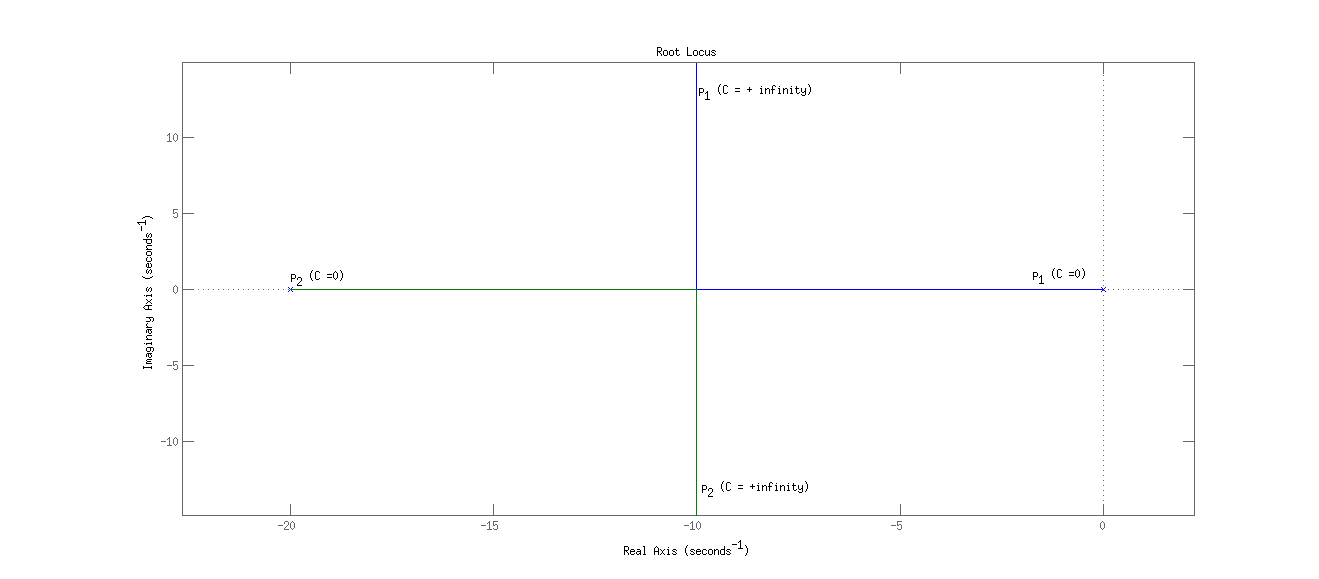
\includegraphics[scale=0.4]{rlocus.png}
\caption{Lieu des pôles (simulé sous Matlab avec la fonction \texttt{rlocus})}
\end{figure}

Pour $m<1$, les pôles se déplacent sur un axe vertical. La distance à l'origine ($\omega_0$) et l'angle avec l'axe vertical ($m$) varient donc simultanément.
 
\item À l'aide des abaques, pour $C=C_0$, donc $m=0,8$ et $\omega_{0BF} = 12,5 rad/s$, on obtient :
\[t_r = 280 ms \]
\[D_1 = 1,5\% \]

Le gain statique de la fonction de transfert en boucle fermée est unitaire, donc l'erreur statique de position est nulle.
\end{itemize}

\subsection*{Manipulation 2}

\begin{itemize}\setlength{\itemsep}{10mm}
\item Avec les paramètres trouvés en préparation 1, on recalcule :
\[ C_0 = 1,485 \quad \et \quad \omega_{0BF} = 11,16 rad/s \]
On a alors
\[ t_r = 313 ms \quad \et \quad D_1 = 1,5\% \]

\item Lorsqu'on applique un échelon au système bouclé, on observe deux phases dans la réponse. En effet, il y a un jeu important dans l'engrenage, c'est le phénomène qu'on observe en premier. Ce phénomène a également tendance à retarder la réponse. Pour le minimiser, on augmente l'amplitude de la consigne.\\

Sur l'\emph{annexe 5}, on relève la réponse de $v_{\theta}(t)$ à un échelon de consigne. On observe un temps de réponse de $394ms$. C'est plus élevé que ce à quoi on s'attendait car il y a du jeu dans l'engrenage qui peut retarder la réponse. L'erreur statique est quasiment nulle.

Le dépassement prévu était de l'ordre de $1\%$ donc n'est pas visible sur le relevé.

\item Sur les faibles amplitudes, l'erreur statique augmente (voir \emph{annexe 6}). En effet, le phénomène de jeu ainsi que celui de frottement sec ne sont plus négligeables et le modèle de second ordre n'est plus valable.


\item \textbf{Régime harmonique}

On veut déterminer le coefficient $m$ et la pulsation propre $\omega_{0BF}$ du système bouclé.\\

Pour cela, on va chercher la pulsation pour laquelle le déphasage est de $90^o$ ($\omega=\omega_{0BF}$). Ainsi, on aura un gain de $\frac{1}{2m}$. (\emph{Annexe 7})

On obtient ce déphasage pour $\omega_{0BF}=11,74Hz$, ce qui est conforme à ce qu'on attendait. (11,16Hz)
Le gain est de -3.3dB donc on obtient $m=\frac{1}{2}10^{3,3/20}=0.73$. (valeur attendue de 0,8)

\item Grâce à cette manipulation, on peut conclure que le modèle de second ordre pour la réponse en angle est valable dans un domaine d'amplitude de consigne élevée. Lorsque l'amplitude est faible, des phénomènes (jeu dans les engrenages, frottement sec) interviennent et mettent à mal le modèle.
\end{itemize}
\section*{IV/ Asservissement de position par retour d'état}

\subsection*{Préparation 3}

\begin{itemize}\setlength{\itemsep}{10mm}
\item On part de la fonction de transfert
\[ \frac{V_{\theta}(p)}{U(p)} = \frac{K_2}{p(1+\tau p)} \]
On a donc
\[\boxed{K_2 u(t) = \frac{dv_{\theta}(t)}{dt} + \tau \frac{d^2v_{\theta}(t)}{dt^2}} \]

\item En posant
\begin{align*}
& \left\{
\begin{array}{ll}
x_1(t) & = v_{\theta}(t) = y(t) \\
x_2(t) & = \frac{dv_{\theta}(t)}{dt}
\end{array}
\right.
\intertext{on a alors}
& \left\{ 
\begin{array}{ll}
\frac{dx_1(t)}{dt} & = x_2\\
\frac{dx_2(t)}{dt} & = \frac{K_2}{\tau}u(t) - \frac{1}{\tau}x_2(t)
\end{array}
\right.
\end{align*}

Le modèle d'état peut donc s'écrire sous forme canonique commandable :
\[
\left\{ 
\begin{array}{rl}
\frac{d}{dt} \left[\begin{array}{c}
x_1(t) \\
x_2(t)
\end{array} \right]
 & = \left[\begin{array}{cc}
0 & 1 \\
0 & -\frac{1}{\tau}
\end{array} \right]
.
\left[\begin{array}{c}
x_1(t) \\
x_2(t)
\end{array} \right] + \left[\begin{array}{c}
0 \\
\frac{K_2}{\tau}
\end{array} \right] u(t) \\
\\
y(t) & = \left[\begin{array}{cc}
1 & 0\\
\end{array} \right]. \left[\begin{array}{c}
x_1(t) \\
x_2(t)
\end{array} \right]
\end{array}
\right.
\]

\item En posant $u(t) = -Lx(t) + \eta e(t)$, avec $L=[l_1 \quad l_2]$, 
\begin{align*}
\frac{d}{dt} \left[\begin{array}{c}
x_1(t) \\
x_2(t)
\end{array} \right]
 & = \left[\begin{array}{cc}
0 & 1 \\
0 & -\frac{1}{\tau}
\end{array} \right]
.
\left[\begin{array}{c}
x_1(t) \\
x_2(t)
\end{array} \right] + \left[\begin{array}{c}
0 \\
\frac{K_2}{\tau}
\end{array} \right] (-\left[\begin{array}{cc}
l_1 & l_2
\end{array}\right]x(t) + \eta e(t)) \\
\\
& = \left[\begin{array}{cc}
0 & 1 \\
-\frac{K_2l_1}{\tau} & -\frac{K_2l_2 +1}{\tau}
\end{array} \right]
.
\left[\begin{array}{c}
x_1(t) \\
x_2(t)
\end{array} \right] + \left[\begin{array}{c}
0 \\
\eta \frac{K_2}{\tau}
\end{array} \right] e(t))
\end{align*}

On a donc
\[ \boxed{F = \left[\begin{array}{cc}
0 & 1 \\
-\frac{K_2l_1}{\tau} & -\frac{K_2l_2 +1}{\tau}
\end{array} \right] \quad \et \quad G = \left[\begin{array}{c}
0 \\
\eta \frac{K_2}{\tau}
\end{array} \right] } \]

\item Calculons l'équation caractéristique $D(p)= det(pI-F)$ du système bouclé :

\[ D(p) = det
\left[\begin{array}{cc}
p & -1 \\
\frac{K_2l_1}{\tau} & p+\frac{K_2l_2 +1}{\tau}
\end{array} \right] \]
\[\boxed{D(p) = p^2 + \frac{K_2l_2 +1}{\tau}p + \frac{K_2l_1}{\tau}}\]

On peut l'assimiler à l'équation caractéristique d'une fonction de transfert du second ordre :
\[D_{2nd}(p) = p^2 + 2m_{BF}\omega_{0BF} + \omega_{0BF}^2\]

avec
\begin{align*}
2m_{BF}\omega_{0BF} & = \frac{K_2l_2 +1}{\tau} \\
\omega_{0BF}^2 & =  \frac{K_2l_1}{\tau}
\end{align*}
Ainsi,
\[ \boxed{ l_1 = \frac{\tau \omega_{0BF}^2}{K_2} \quad \et \quad l_2 = \frac{2\tau m_{BF} \omega_{0BF}-1}{K_2} } \]

On veut un amortissement $m_{BF} = 0.8$ et $\omega_{0BF} = $ 20 puis 30 et 50 rad/s :\\

\begin{center}
\begin{tabular}{|c|c|c|}
\hline 
$\omega_{0BF}$ & $l_1$ & $l_2$ \\ 
\hline 
20 & 4.17 & 0.125 \\ 
30 & 9.38 & 0.292 \\ 
50 & 26.0 & 0.625 \\ 
\hline
\end{tabular}
\end{center} 

\item On a $u(t) = -[l_1 \quad l_2]x(t) + \eta e(t)$ et on veut une erreur statique d'asservissement nulle, c'est-à-dire que $u(\infty) = 0$ lorsque $v_{\theta}(\infty) = e(\infty)$ : il faut donc que $\eta = l_1$.

\subsection*{Manipulation 3}
\begin{itemize}\setlength{\itemsep}{10mm}
\item On met en oeuvre la correction par retour d'état en utilisant un gain $\frac{l_2K_{\theta}}{K_{\Omega}}$ pour $V_{\Omega}$ et $l_1$ pour $V_{\theta}$.

On effectue, pour chacune des valeurs de $\omega_{0BF}$, une réponse à un échelon et une réponse harmonique.
\begin{figure}[h!]
\centering
\begin{tabular}{|c|c|c|c|c|c|}
\hline 
$\omega_{0BF}$ (rad/s) & erreur statique & $D_1$ & $t_{r5}$ (ms) & $m_{BF}$ & Relevé \\ 
\hline 
20 & 0 & 1  \% & 150 & 0.64 & 8 et 9 \\ 
\hline 
30 & 0 & 7 \% & 99 & 0.54 & 10 et 11 \\ 
\hline 
\end{tabular} 
\end{figure}

Pour $\omega_{0BF}=50rad /s$, la réponse en régime harmonique n'est plus sinusoïdal (\emph{Annexes 12 et 13}). Des effets non linéaires apparaissent et on ne peut plus du tout utiliser le modèle du second ordre.

On voulait imposer $m=0,8$ mais on observe que $m$ diminue. En effet, on avait considéré que le modèle était un second ordre. En réalité, lorsque $\omega_{0BF}$ augmente, on se rapproche de l'influence du système mécanique, ce qui rajoute encore de la phase. 

Par conséquent, la marge de phase du système diminue, et donc $m$ diminue et les dépassements augmentent.\\

Au delà de 20 rad/s, les performances sont fortement impactées par les effets de non linéarité du système.
\end{itemize}

\end{itemize}

\section*{Conclusion}
Nous avons au cours de ce TP identifié le moteur à l'aide d'une approche temporelle et harmonique. Nous avons ensuite vu que la correction proportionnelle classique permettait de garantir certaines performances, mais pas de régler indépendamment $\omega_{0BF}$ et $m_{BF}$. Ainsi, la mise en place de la commande par retour d'état permet, dans un certain domaine de validité, de régler ces paramètres de manière indépendante.
\end{document}